%!TEX root = ../Report.tex
%************************************************
\chapter{Music and music-representation}\label{ch:introduction}
\section{Musical elements}
Music is an art form for which the medium is sound.
The common elements in music are:
\begin{itemize}
\item Pitch - Subjective sensation reflecting lowness and highness of sound, also represented more objectively as frequency.
\item Rhythm - Arrangement of sounds and silences.
\item Dynamics - Execution of a given piece (speed, volume)
\item Timbre - Tone
\end{itemize}

Music composition refers to the creation and recording of music through a medium that others can interpret.  Music can be composed for repeated playback or it can be composed on the spot.

A melody is a set of notes (or rests) that are performed in series. Each note may have a different length and different stress. These notes are arranged in a certain rhythmic pattern.

Notes were traditionally given a letter to represent the pitch of the note. The names come from the set $\{A, B, C, D, E, F\}$. Notes may have their pitch modified by additional symbols such as a sharp($\#$).

Notes and rests may have different lengths.


Li and Sleep have found that a given piece of music remains recognizable when the length of the notes are randomized \cite{Ling2004}.

\section{Midi}
Music can be stored digitally in a variety of formats and encodings. This allows repeated performance of the same track and also eases distribution of the music.

\ac{MIDI} is a standard which describes the protocol, digital interface and connectors that allows electronic instruments to communicate with one another.

The \ac{MIDI} 1.0 detailed specification fully describes the \ac{MIDI} interface \cite{MIDIManufacturersAssosciation1995}

The \ac{MIDI} file format describes the way \ac{MIDI} information is stored in a file. Each \ac{MIDI} file starts with a header chunk that describes the time division and the number of tracks. After the header chunk multiple track chunks occur. Each track contains multiple \ac{MIDI} events.

The header chunk is described as follows:
\begin{lstlisting}
"MThd" + [header_length] + [format] + [n] + [division]
\end{lstlisting}
where
\begin{acronym}
\item{[header\_length]} always 6 bytes
\item{[format]} 0 - single track format, 1 multiple track format, 2 multiple song format
\item{[n]} number of track chunks
\item{[division]} unit of time for delta timing
\end{acronym}

After the header chunk [n] track chunks follow.
Each track chunk is composed as follows:
\begin{lstlisting}
"MTrk" + [length] + [track_event] <+ [track_event1] + [track_event2] + [...] + [track_eventn]>
\end{lstlisting}
where
\begin{acronym}
\item{[length]} number of bytes in track chunk
\item{[track\_event]} sequenced track event, described next
\end{acronym}

The track chunk can be seen to contain multiple track events.
Each track event consists a delta time and either a midi event, meta event or sysex\_event:
\begin{lstlisting}
[v_time] + [midi_event] | [meta_event] | <sysex_event>
\end{lstlisting}
The meta-event contains additional information such as text which can be displayed, instrument names, lyrics and so on.

% Table generated by Excel2LaTeX from sheet 'Sheet1'
\begin{table}[htbp]
  \centering
  \caption{Table containing some midi events}
    \begin{tabular}{rrrrr}
    \toprule
    \multicolumn{1}{c}{\textbf{Command}} & \multicolumn{1}{c}{\textbf{Meaning}} & \multicolumn{1}{c}{\textbf{parameters}} & \multicolumn{1}{c}{\textbf{param 1}} & \multicolumn{1}{c}{\textbf{param 2}} \\
    \midrule
    0x80  & Note-off & 2     & key   & velocity \\
    0x90  & Note-on & 2     & key   & velocity \\
    0xA0  & Aftertouch & 2     & key   & touch \\
    0xB0  & Continuous controller & 2     & controller \# & controller value \\
    0xC0  & Patch change & 2     & instrument \# &  \\
    0xD0  & Channel Pressure & 1     & pressure &  \\
    \bottomrule
    \end{tabular}%
  \label{tab:midievents}%
\end{table}%

Table \ref{tab:midievents} shows some of the possible midi events. Each event has a command and additional arguments.

The full midi specification can be ordered online at \href{http://www.midi.org/}{midi.org}\footnote{http://www.midi.org/}


\section{Representation}
Representation of music is important to achieve successful generation of a correct solution \cite{gibson1991neurogen}. However the search space of machine learning algorithms may be too large if limitations are not introduced \cite{Jacob1995}. 

The musical data from musical pieces need to have a proper representation in order to be used by a machine learning algorithm.

In \cite{Eck2002} Eck a form of 12-bar blues was used with 8 notes per bar. 
He used the following representation for the \acs{LTSM} system:
\begin{enumerate}
\item 12-bar musical pieces were used
\item 8 notes per bar were used
\item The same chords were used between songs, see figure \ref{ims:eckchords}
\item The melody notes were built using the pentatonic scale
\item The neural network inputs indicate whether a certain note is on or off
\end{enumerate}

A melody would be represented differently in a linear genetic algorithm.
A simple melody consisting only of a few notes could be represented as seen in figure \ref{ims:ga_melody}. Note the duration of a note is not defined and could be consider fixed.

However it might be preferably to encode more events such rests, chords, dynamics, note duration and so on.

Tree based representations are found in genetic programming \cite{Langdon2008}. Minsky has argued that tree representation is more suited to music as it mimics the hierarchical structure that is found in music \cite{Minsky1992}.

A melody could be represented in tree form as seen in figure \ref{ims:gp_melody}. The bottom leaves denote the pitch and duration. The higher level nodes perform operations.


\begin{figure}
\centering
\begin{minipage}{.5\textwidth}
  \centering
  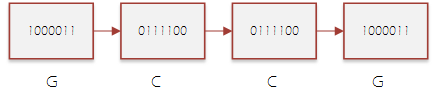
\includegraphics[width=180px]{../images/ga_melody.png}
  \caption{Simple melody represented as a bit string}
\label{ims:ga_melody}
\end{minipage}%
\begin{minipage}{.5\textwidth}
  \centering
  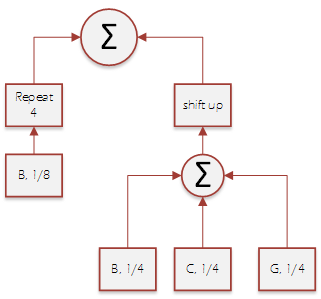
\includegraphics[width=180px]{../images/gp_melody.png}
  \caption{Simple melody represented in tree form}
\label{ims:gp_melody}
\end{minipage}
\end{figure}

\begin{figure}
\centerline{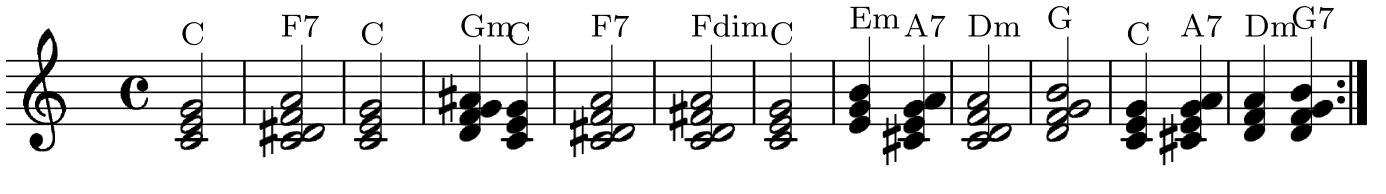
\includegraphics[width=400px]{../images/eck_chords_training.png}}
\caption{Training chords used in \cite{Eck2002}}
\label{ims:eckchords}
\end{figure}

Johanson and Poli employ several different operators including mirroring, concatenation, repetition and mirroring \cite{Johanson1998}

Tree based representations do not have a fixed size, as is commonly found in linear genetic representations. Care must be taken to not let the structure become too large. This is typically done by specifying the maximum depth of the tree.

%********************************************************************************************************
%********************************************************************************************************
%********************************************************************************************************

\chapter{Music composition algorithms} \label{chap:comp_algo}



%\section{Harmony Search Algorithm}
%Music pieces have been composed using a behavior-inspired evolutionary algorithm, harmony search (HS). The HS algorithm mimics behaviors of music players in an improvisation process, where each player produces a pitch based on one of three operations (random selection, memory consideration, and pitch adjustment) in order to find a better state of harmony which can be translated into a solution vector in the optimization process. When HS was applied to the organum (an early form of polyphonic music) composition, it could successfully compose harmony lines based on original Gregorian chant lines.

%****************************************************************************************************

\section{Neural Networks}
\subsection{Background}
\begin{figure}
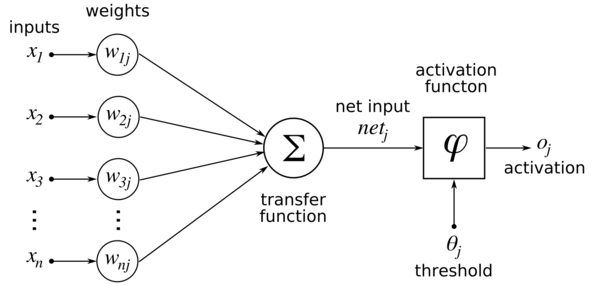
\includegraphics[width=300px]{../images/ANN_neuron.png}
\caption{Model of artificial neuron}
\label{ims:ANN_neuron}
\end{figure}
\begin{figure}
\centerline{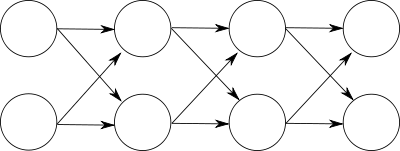
\includegraphics[width=200px]{../images/ANN_feedforward.png}}
\caption{Figure of ANN in feed-forward topology}
\label{ims:ANN_FF}
\end{figure}
An artifical neural networks consists of layers of artificial neuron\footnote{neurons are commonly referred to as units} (see figure \ref{ims:ANN_neuron}) that are connected to each other in a certain topology \cite{bishop1995neural}.

Figure \ref{ims:ANN_FF} shows a multilayer ANN in feed-forward topology. The first layer is referred to as the input layer, the right-most layer is referred to as the output layer, the layers in between the input layer and the output layer are known as hidden layers.

Neurons have a number of inputs which are summed into an activation function. The activation function provides the output of a neuron.
In figure \ref{ims:ANN_neuron} we have
\[ o_j = \varphi(\sum^{n}_{i=1} x_i w_{ij})  \]
A common activation function is the continous sigmoid function given by
\begin{equation} \varphi(t) = \sigma(t) = \frac{1}{1+e^{-\beta t}}  \label{eq:sigmoid}\end{equation}
where $\beta$ is the slope parameter.
The derivative of the sigmoid function is easy to obtain and is given by:
\begin{equation} \frac{\sigma(t)}{dt} = \sigma(t)(1-\sigma(t))\label{eq:sigmoidd}\end{equation}
for $\beta=1$

In order to determine weights for a two-layer neural network we need to minimize the error between the output of the neural network and the given target value for a set of inputs. 

Thus for the output neurons we have
\begin{equation} E(\vec{w}) = \frac{1}{2} \sum_{d \in D}(t_d - \sigma_d)^2 \label{eq:error} \end{equation}\
where $D$ is the set of training examples and $t_d$ is the target output for training example $d$ and $o_d$ is the output of the artificial neuron for training example $d$
We need to minimize equation \ref{eq:error}.
Obtaining the deriviative of $E$ with respect to $w_i$ yields:
\[ \frac{\partial E}{\partial w_i} = \sum_{d\in D}(t_d - o_d)(-x_id) \]
where $x_{id}$ is the input for component $x_i$

Gradient descent is a optimization algorithm that takes steps proportional to the negative of the gradient. This we update the weights by:
\[\vec{w} \leftarrow \vec{w} - \eta \nabla E(\vec{w}) \]
Applying the gradient descent algorithm we obtain a weight update rule of
\[ w_i \leftarrow w_i + \eta \sum_{d \in D} (t_d - o_d) x_{id} \]
For a multi layer network with multiple output units the back propagation algorithm needs to be used.
The error needs to be summed over all the network output units
\[E(\vec{w}) = \frac{1}{2} \sum_{d \in D} \sum_{k \in \text{outputs}} (t_{kd} - \sigma_{kd})^2 \]

The backpropagation algorithm to determine the weights of a feed-forward neural network is given in appendix \ref{chap:app_algo}


\subsection{Composition}
Neural networks have been used in music classification, in genetic algorithms as fitness functions and more complex neural networks have even been used in algorithmic music compositions.

Simple feed-forward neural networks do not contain a mechanism to remember past history.  
\\
\\
In \cite{mozer1994neural} Mozer created a recurrent connectionist neural network \textbf{CONCERT}\footnote{CONCERT - connectionist composer of ERudite tunes}\footnote{The ER may also be read as ERratic or ERsatz}.
The system works as follows:
\begin{itemize}
\item The network is trained on sample melodies from which it learns melodic and phrase constraints
\item Representations of pitch, duration and harmonic structure that are based on psychological studies of human perception, based on Laden and Keefe's work \cite{laden1989representation}
\end{itemize}
The system yielded good results on simple structured artificial sequences however the system performed poorly on natural music\footnote{One critic described the resultant melodies as compositions only a mother could love}. Mozer described the system as lacking musical coherency \cite{mozer1994neural}. Furthermore the system performs poorly as the length of the pieces increases.

Mozer stated the reason for failure is likely due to the \ac{RNN} not being able to track more distant events that build global structure \cite{mozer1994neural} however a \ac{LTSM} recurrent network is able to achieve this goal \cite{Eck2002}.
\\
\\
In order to solve the problem of global structure Douglas and Jurgen attempted to use a \textbf{\ac{LTSM}} network to compose musical pieces \cite{Eck2002}. In this attempt the network was successfully able to learn a form a blues music and stay close to the relevant structure.
The system used cross entropy as the error rate:
\[
E_i = -t_i \ln(y_i) - (1-t_i)\ln (1-y_i) \]
where $y_i$ is the output activation and $t_i$ the target value for the $i-th$ output unit.
The topology of the network was arranged as follows:
\begin{enumerate}
\item Four cell blocks are connected to the input units for chords
\item The last four cell blocks are connected to the inputs units for melody
\item chord cell blocks have recurrent connections to themselves and melody cell blocks
\item melody cell blocks have recurrent connections to other melody cell blocks
\item output units for chords are connected to cell blocks for chords and to input units for chords
\item output units for melody are connected to cell blocks for melody and to input units for melody
\end{enumerate}
The underlaying chord structure was kept fixed.

The results indicate that a \ac{LTSM} network is able to compose with both local- and global structure from a set of training data \cite{Eck2002}.


\subsection{Conclusion}

Simple feed-forward neural networks do not have the functionality to remember past history and thus do not have the capability to evaluate repetitive rhythmic patterns.

Recurrent neural networks are able to encode temporal information though initial investigation by Mozer lead to limited success as compositions lacked global structure. 

Further investigations by Douglas and Jurgen indicated that \ac{LTSM} networks are able to compose with local and global structure.

%****************************************************************************************************
\section{Genetic Algorithms}
\subsubsection{Background}

Genetic Programming, not to be confused with evolutionary or genetic algorithms is a evolutionary algorithm based methodology to find computer programs that perform defined tasks by simplistically mirroring biological evolution.
The more fit programs carry on their chromosomes into future populations. Fitness is rated by a fitness function. Other genetic operators such as recombination and crossover are also usually applied. 
These evolved genetic programs are usually represented in tree form. Figure \ref{ims:gpt} indicates the function $ (2.2) - (\frac{X}{11}) + 7\cos(Y)$ written in tree form.
\begin{figure}[!bh]
\centerline{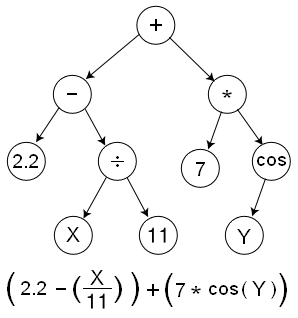
\includegraphics[width=150px]{../images/gpt.png}}
\caption{Figure of a example genetic program tree}
\label{ims:gpt}
\end{figure}

A genetic algorithm consists of the following components:
\begin{enumerate}
\item Representation for chromosomes\footnote{Also commonly referred to as an individuals}
\item Initial population of chromosomes
\item A set of genetic operators to alter the population
\item A fitness function to assess the fitness of an individual
\item A selection method to determine which individuals in a population survive
\end{enumerate}
The algorithm proceeds as follows:
\begin{enumerate}
\item Initial population is randomly generated
\item The fitness of each individual is assessed
\item Individuals are selected to which genetic operators are applied, e.g.
\\Two parents are selected to generate a new child with crossover
\\Random mutation occurs in individual
\item Various forms of selection are available that determine which individuals will be in the next generation
\end{enumerate}

\textbf{Genetic operators} are used to generate diversity A genetic algorithm has a fixed set of genetic operators. Operators may include:
\begin{itemize}
\item Reproduction - A parent from the population is carried over to the next generation
\item Crossover - genotype of both parents are combined using different procedures
\item Mutation - A single mutation is applied to a chromosome at a set mutation rate
\end{itemize}

The choice of a \textbf{fitness function} is a big problem when using a genetic algorithm to compose music \cite{Wiggins1998,Matic2010}. There is no objective method to rate whether a melody is good or bad \cite{Lo2012}. 
Traditionally when posed against such tasks the fitness function is provided interactively by the user, i.e. the user rates whether the piece is good or bad

The interactive GA approach is an approach to the fitness function where a human interactively rates the quality of a composition (fitness). A well known software that utlizes a neural network and a interactive interaction for a fitness function is GenJam \cite{Biles1996}. The drawback of having the user interactively evaluate the fitness of individuals is that it is time consuming and poses a processing bottleneck \cite{Eck2002}

\textbf{Selection} is the choice of which individuals will be chosen for the next generation. Selection concerns the reproduction and crossover operators. Some methods of selection include: 
\begin{itemize}
\item Roulette wheel selection - chance of individual being chosen is proportional to fitness
\item Tournament selection - tournament is staged between two individuals to detemine which one gets selected\footnote{This is tournament selection in its simplest form}.
\end{itemize}

\subsubsection{GA approaches to music composition}

Genetic algorithms have already been used in a variety of work in algorithmic music composition. Some of these include:
\begin{itemize}
\item Thematic bridging \cite{Horner1991}
\item Composition systems using \acsp{IGA} \cite{1412045}
\item \acsp{IGA} to improvise jazz solos \cite{Biles1996, Biles1994}
\item Integration between interactive genetic algorithms and genetic programs \cite{Tokui2000}
\item Hybrid approaches employing statistical, connectionist and evolutionary elements \cite{Manaris2007}
\item Various work into different fitness functions
\end{itemize}

In \cite{Alfonseca2007} the generated musical pieces had the style of well-known authors even when the fitness function only took relative pitch envelope into account and all generated note lengths were of fixed duration.
\\
\\
\textbf{Thematic bridging} is the application of an initial music pattern to a final pattern over a specified duration \cite{Horner1991}. In this approach Horner modified or reordered elements in a music pattern through various operations. For example:

Given the initial note pattern of:
 \begin{verbatim}Gb Bb F Ab Db \end{verbatim}
and a final note pattern of:
\begin{verbatim}F Ab Eb \end{verbatim}
the musical output could be:
\begin{verbatim}Gb Bb F Ab Bb F Ab Gb Bb F Ab Eb F Ab F Ab Eb \end{verbatim} by means of various operations such as mutation, rotation, deletion and so on.
For thematic bridging a composite fitness function was used which rates how close the developed pattern matches the final pattern and whether the ordering of the elements are correct 
\\
\\
Similarly a system of \textbf{variations} was developed Jacob that proceeds as follows \cite{Jacob1995}:
\begin{enumerate}
\item Define a primary set of motives
\item Compose phrases by layering and sequencing new motives
\item New motives are created by variations of motives already in the phrase
\item Phrases are combined together
\end{enumerate}
Jacob's system had a human judge evaluate the individual chromosomes. 
\\
\\
\textbf{\ac{NCD}} has also been commonly used as a fitness function, for more information about the normalized compression distance see sections \ref{sec:class_ncd} (in music classification) and \ref{sec:ncdfitness} (as a fitness function).
Alfonseca proposed the following genetic algorithm scheme for composing melodies \cite{Alfonseca2007}:
\begin{enumerate}
\item Define a set of $M$ musical pieces for a guide set $G$
\item Encode both the guides and individuals in the population as pairs of integers where the first integer represents the note interval and the second the length as a multiple of the minimum unit of time.
\item See eq. \ref{eq:ncdfitness} on page \pageref{eq:ncdfitness} for the fitness function used
\item The 16 lowest fitness genotypes of every generation is removed
\item The 16 highest fitness genotypes of every generation are paired by means of genetic operations.
\end{enumerate}


\subsubsection{Conclusion}
There are various variations on genetic algorithms and genetic programs, however evolutionary algorithms are a viable means to compose music.

The encoding of a musical piece as a chromosome affects the interactions of the genetic operators on the musical piece and most authors encode the problem differently.

It is important to restrict the domain of problem otherwise the search space for the genetic algorithm may be too large \cite{Jacob1995}. Most of the studies listed in this document had restricted goals.
For example, using only two octaves for the notes significantly reduces the size of the search space and many real melodies comply with it \cite{Alfonseca2007}

The fitness function is an important part for having the genetic algorithm result to good melodies. See section \ref{sec:chapfitness} for insight literature has on fitness function for evolutionary algorithms.
The representation of melodies for the algorithm is arguably just as important.

For this project the focus is on evolutionary algorithms and as such other procedural means of music composition will be neglected. There is too much work in music classification and as such the focus will be on only a few possible algorithms.

Fitness functions for genetic algorithms are considered in chapter \ref{sec:chapfitness}


%********************************************************************************************************
%********************************************************************************************************
%********************************************************************************************************

\chapter{Music classification} \label{sec:music_class}
\section{Introduction}
In this section we will investigate methods of music classification. If some algorithm is a good method to rate the closeness of a song to a genre or style then it may also serve as a good fitness function for a evolutionary algorithm.
%\section{Feature set patterns}
%Melody classification using patterns
%Darrell Conklin
%Abstract. A new method for symbolic music classification is proposed,
%based on a feature set pattern representation. An ensemble of sequential
%patterns is used to classify unseen pieces using a decision list method.
%On a small corpus of 195 folk song melodies this method achieves a good
%classification accuracy of 77\%, though with only a 43\% recall rate.


\section{Normalized Compression Distance} \label{sec:class_ncd}
\subsection{Background}
The Kolmogorov complexity of piece of text is the measure of the computable resources needed to specify the text. The complexity of a string is the length of the shortest possible description of the string in a fixed universal description langauge \cite{Kolmogorov1998387}.

The information distance between two string $x$ and $y$ is defined as the length of the shortest program $p$ that can compute $x$ from $y$ and $y$ from $x$
The length of $p$ can be expressed using Kolmogorov complexity \cite{681318}:
\[ |p| = \max\{K(x|y), K(y|x)\}  \]

The information distance $p$ is a absolute measure. A more useful similarity metric is one that expresses the distance in relative terms. 
The \ac{NID} is given by \cite{1362909} : 
\[ \text{NID}(x,y) = \frac{\max\{K(x|y),K(y|x)\}}{\max\{K(x),K(y)\}} \]

The concept of \ac{NID} is important, however it is not computable. 
An approximation of the normalized information distance is commonly used.  $K(x)$ is approximated by $Z(x)$ where $Z(x)$ is the binary length of a data $x$ compressed by a compressor $Z$.
\[NCD(x,y) = \frac{Z(xy) - \min\{ Z(x), Z(y) \}}{\max\{ Z(x), Z(y) \}} \]
where $Z(xy)$ is the length of $x+y$ compressed by $Z$. 
Any good compressor may be used for $Z$ such as 
\begin{itemize}
\item gzip
\item bzip2
\item Lempel-Ziv and its variations
\end{itemize}
\subsection{Literature}
Normalized compression distance has been used in a variety of cases. It has been used in applications of general clustering and classification of data in arbitrary domains. This includes music classification \cite{1412045}.

Cilibrasi and Vitiyani used the Normalized Compression Distance to approximate the Kolmogorov Distance between different musical pieces as a method to compute clusters of music \cite{1412045}. The \ac{MIDI} files were pre-processed such that when two notes occur at the same time only the note with the highest pitch is kept. The music was represented as a string and the distances between different musical pieces was computed.


Ctaltepe, Sonmez and Adali used the normalized compression distance and used it to classify music pieces using k-nearest neighbors \cite{Cataltepe2005}. 
The training data has a label associated. The closest $k$ training data (by \ac{NCD}) to a song is obtained and the most frequent label in the $k$ set is used to classify the musical piece. 
Ctaltepe Sonmez and Adali found that the distance measure works better when more training data is available and the performance is dependent on how the input data is pre processed. 
The best results were obtained when the midi files were sampled at $1$ms and the $k=1$ nearest neighbor identification was used. 
The music was represented in the following format: outputting the first note and then the difference in pitch between consecutive notes. Using the above means a classification accuracy of $79\%$ was achieved on 57 midi files.

Li and Sleep have also found that the 1-nearest neighbor with a Lempel-Zip compressor outperformed more complex statistical methods and compressors. Using relative pitch intervals in the music representation outperformed using absolute pitches. A performance of $92.35\%$ was obtained \cite{Ling2004}.
The midi files were organized into four categories Beethoven (302 files), Haydn (261 files), Chinese (80 files) and Jazz (128 files). The dataset is unbalanced and the study does not make it clear which partition of the dataset was used as training samples and what partition was used for verification.

In \cite{Alfonseca2007, Alfonseca:2005:ECM:1981094.1981161, Ling2004,Alfonseca2006} it was found that the normalized compression distance serves as a promising fitness function for genetic algorithms for automatic music generation. Thus \ac{NCD} may be viably used as a fitness function for a genetic algorithm and as a metric to help classify music.

\section{Neural Networks}
McKay investigate using K-nearest neighbor techniques and artificial neural networks in order to classify \ac{MIDI} music by genre.
He included some of the following metrics as input to the neural network \cite{Mckay2004}:
\begin{itemize}
\item Number of notes - standard deviation of number of notes activated in each channel
\item Note duration - standard deviation of total duration of notes
\item Dynamics - standard deviation of average volume of notes
\item Melodic Intervals - average melodic interval
\item Simultaneity - average number of notes that are played concurrently
\item Note density - average number of notes per second
\item Average time between attacks - average time between note activations
\item Initial tempo - tempo in beats per minute
\item Pitch variety - number of pitches used at least once
\item Most common pitch class - Most common pitch divided by number of possible pitches
\end{itemize}
For a full list please see his MacKays dissertation on MIDI classification \cite{Mckay2004}
Using the complete list of metrics neural networks had a success rate of $83\%$.
%********************************************************************************************************
%********************************************************************************************************
%********************************************************************************************************

\chapter{Fitness Functions}\label{sec:chapfitness}

%********************************************************************************************************

\section{Introduction}
In this section we will briefly review some functions that may be used as a fitness function for a genetic algorithm.

%Some other functions that may be used, but with mixed results are identified in section \ref{sec:other} briefly.

Algorithms that help classify music could possibly be used as fitness functions, as this would rate the similarity of the evolved piece of music to a genre or style. These algorithms are found in section \ref{sec:music_class}.
If work has been done that has used the music classification algorithm as a fitness function it will be listed in this section.

Fitness functions can be categorized as follows:
\begin{itemize}
\item Interactive - The user provides the fitness of a piece of music
\item Expert systems - The musical fitness is assigned according to best practices commonly studied in music theory
\item Learning based functions - Fitness functions that learn from previous data
\end{itemize}

Learned fitness functions are sensitive to input data and the selection of features is a difficult task \cite{Dostal2013}.
%********************************************************************************************************


\section{Zipf's law} \label{sec:zipfs_fitness}
Zipf's law states that the frequency of an event is inversely proportional to its statistical rank, that is:
\[ f \propto r^{-a} \]
where $f$ is the frequency of occurence of a particular event and $r$ is the statistical rank. $a$ is close to $1$.
Zipf's law can also be stated as:
\[ P(f) \approx \frac{1}{f^n}\]
where $P(f)$ denotes the probability of an event of rank $f$ and $n$ is close to $1$

One can determine whether melodic intervals follow Zipf's law by counting the melodic intervals in a piece. The result is usually plotted on a logarithmic scale and is known as a rank-frequency distribution

Zipf found evidence for the theory in music. An analysis of Mozart's Bassoon Concerto in Bb Major revealed an inverse relationship between the length of intervals between repetitions of notes and the frequency of their occurrence \cite{zipf1949human}.

Several other different rank frequency distributions can be obtained for a musical piece.
These include \cite{Manaris2005}:
\begin{itemize}
\item{Pitch}{ - distribution of \ac{MIDI} pitches}
\item{Chromatic tone}{ - distribution of 12 chromatic tones}
\item{Duration}{ - note durations}
\item{Melodic interval}{ - distribution of melodic intervals}
\item{Melodic bigrams}{ - distribution of adjacent melodic interval pairs}
\end{itemize}
Linear regression is performed to obtain the slope of the distribution. The coefficient of determination $R^2$ is also computed in order to determine how well the slope fits the data.

\begin{figure}
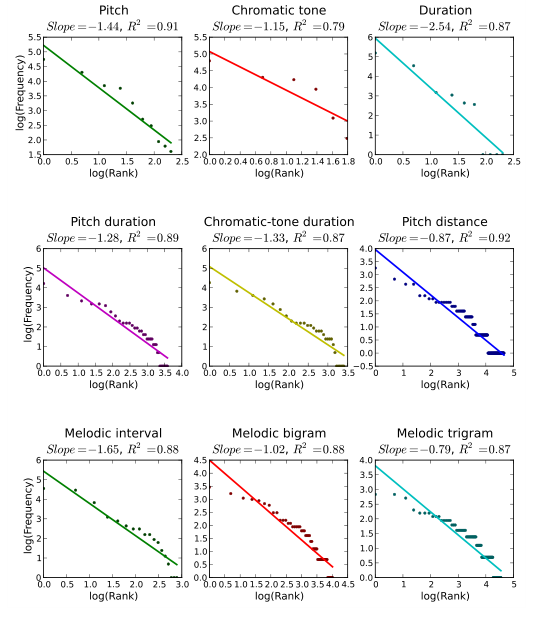
\includegraphics[width=400px]{../images/zipf_letitbe.png}
\caption[Rank frequency distributions for Let It Be]{Rank frequency distributions and slopes of different metrics for The Beatles' Let It Be
\footnotemark}
\label{ims:zipf_letitbe}
\end{figure}
\footnotetext{Figure generated by Jensen for his thesis \cite{Dostal2013}}


Figure \ref{ims:zipf_letitbe} plots the rank frequency distributions of various metrics for the Beatles' song Let It Be. The figures were generated by Jensen for his thesis \cite{Dostal2013}. The metrics can be seen to follow a Zipfian distribution. Results by Manaris also indicate that most music pieces display near Zipfian distributions \cite{Manaris2005}.

Zipf-based metrics capture essential parts of scaling properties in music. These metrics indicate that music follows a distribution balanced between near-zero slope and steep negative slope. Different styles of music have different slopes.
There exists also a correlation between Zipf metrics and human preference \cite{Manaris2005}.

Jensen used a Gaussian to define the target fitness as \cite{Dostal2013}:
\[f_m(a,b) = e^{(\frac{b-a}{-\lambda})^2} \]
where $a$ is the metric slope of an evolved piece of music, $b$ is the target slope and $\lambda$ is the tolerance

Since there are several metrics for a given piece of music the fitness function should incorporate these.
Jensen used the weighted sum of several metrics.  
\[f(\vec{a}, \vec{b}) = \sum_{i=1}^{N} w_i f_i(a_i, b_i) \]

Jensen has found that Zipf metrics can be used to evolve pleasant music using a tree-based representation, however the majority of the evolved melodies were unpleasant \cite{Dostal2013}. Zipf metrics only capture the scaling properties of distributions and ignore the musical events that account for different frequencies. Zipf's law neglects musical content and can be seen as knowledge weak.
Jensen concluded that the Zipf metrics are insufficient for musical fitness alone.

Manaris had more success with Zipf metrics however he used them as input to an artificial neural network to evaluate the fitness of melodies, however Manaris states it is wiser to use the fitness function in a partially interactive system \cite{Manaris2005}

%********************************************************************************************************

\section{Cosine Similarity}
In Information Retrieval cosine similarity is commonly used to asses the similarity of two documents:
\[\text{sim}(\vec{A}, \vec{B}) = cos\theta = \frac{\vec{A} \cdot \vec{B}}{|\vec{A}||\vec{B}|} \]
where $\vec{A}$ and $\vec{B}$ are two document vectors

In order to rate the similarity between music scores features such as pitches and melodic intervals are used.

As with Zipf's law the fitness is the weighted sum of similarity measures:
\begin{equation}f(\vec{A_1}, \ldots, \vec{A_n}; \vec{B_1}, \ldots, \vec{B_n}) = \sum^N_{i=1} w_i f_i (\vec{A_i}, \vec{B_i}) \label{eq:fitcosfit} \end{equation}
The fitness function rates the fitness of the evolved individual with a target piece.

Jensen conducted multiple experiments using the fitness function in equation \ref{eq:fitcosfit}. At first only a single metric was included and thereafter multiple metrics. As more metrics were included the evolved melodies became more similar to the target piece. More pleasant melodies were evolved when the target piece was The Beatle's Let It Go than Mozart's Piano Sonato No. 16. There was no correlation between melody and rhythm.
Metrics included for the fitness function were:
\begin{itemize}
\item Pitch
\item Chromatic tone
\item Melodic interval
\item Melodic bigram
\item Rhythmic interval
\item Rhythmic bigram
\end{itemize}
Jensen concluded that the results obtained by the cosine simalirity fitness function were more pleasant than those obtained by Zipf's law as Zipf's law rates music on scaling properties only \cite{Dostal2013}.

%********************************************************************************************************


\section{Neural Networks} \label{sec:ANN_fitness}
Different forms of networks have been used as a fitness function for evolutionary algorithms.
Some of these include:
\begin{itemize}
\item Adaptive resonance theory neural networks using binary classification patterns \cite{Burton97geneticalgorithm}
\item Recurrent neural networks
\item Cascade correlation neural network designed to reduce GenJam bottleneck \cite{Biles1996}
\end{itemize}

Some common problems with neural networks as fitness functions is that they require a lot of time to be trained, require a good representation for a set of inputs to map to an output and the structure of the neural network is fixed after training \cite{Burton97geneticalgorithm}. 

In \cite{Biles1996} Biles tried to design a cascore neural network to rate musical scores. Since a neural network outputs fitness based on the input parameters the choice of input metrics are important.
Metrics that included the number of new note events in a measure, the number of unique new note events, the size of the maximum interval, the number of changes in a direction between adjacent notes failed to capture the fitness for the \ac{ANN} \cite{Biles1996}.

Biles argues that the reason for this is that humans listen to music in more complex ways and that simple statistical measures fail to capture this. Zipfs law, which only captures the scaling properties of music also yielded poor results as a fitness function for similar reasons \cite{Dostal2013} (See section \ref{sec:zipfs_fitness}). 
\\
\\
An \textbf{\ac{ART} network} has been used as a fitness function whereby a \ac{GA} utilizes clustered representations of rhythm styles to interactively generate rhythm patterns to according to a certain style \cite{Burton97geneticalgorithm}.

An adaptive resonance theory network utilizes unsupervised learning and clustering algorithms to recognize patterns. New clusters are created if a pattern cannot be associated with existing clusters. Another characteristic of \ac{ART} networks is that new training does not cause loss or corruption of old training data \cite{carpenter2010adaptive}

A ART1 network clusters binary vectors. The basic structure of an ART1 network involves (See figure \ref{ims:ANN_art}) :
\begin{enumerate}
\item Input processing field - $F1$
\item Cluster units - $F2$
\item Mechanism to control degree of similarity of patterns in the same pattern
\item weighted bottom-up connections between $F1$ and $F2$ layers
\item weighted top-down connections between $F2$ and $F1$ layers
\end{enumerate}

\begin{figure}
\centering
\includegraphics[width=300px]{../images/ann_ART.png}
\caption{Figure of ART ANN topology}
\label{ims:ANN_art}
\end{figure}

Burton had the \ac{ART} network fitness function operate as follows \cite{Burton97geneticalgorithm}:
\begin{enumerate}
\item Each individual in the population is an input to the \ac{ANN}
\item The network determines the winning cluster
\item The degree of similarity between the individual and the cluster is determined
\item If the degree of similarity is above a certain threshold the individual is added to the cluster
\item If no clusters match the individual closely enough a new cluster is created
\item Fitness is assigned as a degree of similarity to a cluster. 
\end{enumerate}

\textbf{NEUROGEN} is another attempt at using a neural network as a fitness function to compose small diatonic, western, four part harmony compositions.
The system has shown limited success however it was able to produce 4 bars of music \cite{gibson1991neurogen}.
\\
\\
Chen used a \textbf{\ac{SRN}} with composition rules on tonality and rhythm as a fitness function for a \ac{GA} \cite{Chen2001}. The simple recurrent network has an input layer that represents a measure at time $T$ with the output layer representing the measure at time $T+1$.
A recurrent network is used as a single step predictor to compose music. The network predicts notes at $T+1$ using the notes at time $T$. After the network has been trained it can be seeded with inital values to generate novel compositions.
The following constraints were used:
\begin{enumerate}
\item Pitch diversity constraint - number of measures with unique pitch sequences
\item Rhythmic diversity constraint - number of measures with unique signatures
\item Measure density constraint - ratio of number of notes to maximum notes
\item Pentatonic pitch class constraint - number of notes that belong to pentatonic pitch class
\item Cell structure - ratio number of times cell pattern occurs to maximum number of patterns 
\end{enumerate}
The system was able to generate melodies with systematic structure however it lacks global structure. Individual measures sound pleasant and diverse however there is a lacking structure as a whole
%********************************************************************************************************

\section{Normalized Compression Distance} \label{sec:ncdfitness}
As noted in section \ref{sec:music_class} the Normalized Compression Distance has been used to help classify music genres. However Normalized Compression Distance has been explored as a possible fitness function for evolutionary algorithms \cite{Alfonseca2007,Alfonseca:2005:ECM:1981094.1981161,Alfonseca2006}

The fitness function used by Alfonseca et. al for an individual $x$ and a guide set $G$ was defined as \cite{Alfonseca2006}: 
\begin{equation}f(x) = \left( \sum_{g_i\in G} \text{NCD}(x,g_i) \right)^{-1} \label{eq:ncdfitness} \end{equation}
Where $g_i$ is a guide in guide set $G$ containing $M$ musical pieces and $x$ is the set of differences between consecutive notes.

Alfonseca encoded the chromosomes as $N$ vectors containing a pair of integers. The first integer denotes the note interval and the second represents the length as a multiple of the smallest unit of time \cite{Alfonseca2007}.

%********************************************************************************************************

\section{Interactive fitness functions} \label{sec:iga}
Genetic algorithms which employ user interaction as a means of rating the fitness of are known as \acfp{IGA}.

In \cite{Unehara} constructs a system that composes 16-bars music using a GA. The user rates individual chromosomes, new chromosomes are applied by genetic algorithm and the user is asked to rate the individuals again. Should the user find a good piece they may favorite it. The fitness of the chromosomes were seen to increase as the generations increased, however it is unknown whether the melodies were pleasant.

Using an interactive fitness function may lead to better results than most other fitness functions however it is a tedious and demanding process and may also lead to inconsistencies in evaluation.
Some researches try to reduce this effect by constructing \acp{ANN} which learn the user's ratings, and as such may be used in place of the interactive fitness function \cite{Biles1996,Spector_inductionand}. See section \ref{sec:ANN_fitness} for the use of \acp{ANN} as fitness functions.

Johnson and Poli had a user rate individual sequences and trained a neural network base automatic rater, which may replace the user in larger runs. The musical pieces generated by the automatic rater were pleasant but they were not as pleasant as the musical pieces generated by the user interactive runs \cite{Johanson1998}

The superiority of a interactive fitness can be seen, as a person can rate the pleasantness, or fitness of a song much more accurately than current quantitative fitness functions. However this imposes a bottleneck on the system as it is time consuming. A partially interactive system may yield a good compromise \cite{Biles1996}.


\chapter{Conclusion}
We have investigated numerous methods to compose music algorithmically. The two most prominent methods currently to compose music is through genetic algorithms and neural networks.

Genetic algorithms require proper music representation and a good fitness function. Multiple work has gone into investigating various possible fitness functions. The three most promising candidates are \ac{NCD}, \ac{ANN} and cosine similarity.

Interactive genetic algorithms yield good results although this imposes a performance bottleneck on the system, as the system is required to wait for user input. This is a time-consuming process although a partial interactive system might be viable.

Simple feed-forward neural networks are unable to compose music due to their inability to encode temporal information. Recurrent neural networks were investigated and early findings yielded poor results, though LTSM networks seem promising.

Algorithmic music composition is viable although there is large room for improvements to be made. Currently only short musical pieces sound pleasant. Longer pieces tend to be repetitive and lack global structure. 

Most current methods restrict their domain in order to investigate only the main research questions. 

A hybrid approach may yield good results. 

%********************************************************************************************************


%*****************************************
%*****************************************
%*****************************************
%*****************************************
%*****************************************



























\chapter{Notes}
%Tokui constructs the system generating rhythm section (i.e. drum set) [10]. He uses the neural
%network approach to evaluate rhythm section. That is, the neural networks obtained by some learning method
%play the role of fitness functions.